%\newpage
%\thispagestyle{plain}
%\ifthenelse {\boolean{bachelor}}
%{
%	%\section{Technical documentation}
%	\section{Technická dokumentácia}
%}
%{
%	%\chapter{Technical documentation}
%	\chapter{Technická dokumentácia}
%}
% \label{technical_documentation}
%Lorem ipsum dolor sit amet, consectetuer adipiscing elit, sed diam nonummy nibh euismod tincidunt ut laoreet dolore magna aliquam erat volutpat. Ut wisi enim ad minim veniam, quis nostrud exerci tation ullamcorper suscipit lobortis nisl ut aliquip ex ea commodo consequat. 
%\ifthenelse {\boolean{bachelor}}
%{
%	%\subsection{Implementation}
%	\subsection{Implementácia}
%}
%{
%	%\section{Implementation}
%	\section{Implementácia}
%}
%\paragraph{Modul abc}
%Lorem ipsum dolor sit amet, consectetuer adipiscing elit, sed diam nonummy nibh euismod tincidunt ut laoreet dolore magna aliquam erat volutpat. Ut wisi enim ad minim veniam, quis nostrud exerci tation ullamcorper suscipit lobortis nisl ut aliquip ex ea commodo consequat. Duis autem vel eum iriure dolor in hendrerit in vulputate velit esse molestie consequat, vel illum dolore eu feugiat nulla facilisis at vero eros et accumsan et iusto odio dignissim qui blandit praesent luptatum zzril delenit augue duis dolore te feugait nulla facilisi. Nam liber tempor cum soluta nobis eleifend option congue nihil imperdiet doming id quod mazim placerat facer possim assum.
%\paragraph{Modul def}
%Lorem ipsum dolor sit amet, consectetuer adipiscing elit, sed diam nonummy nibh euismod tincidunt ut laoreet dolore magna aliquam erat volutpat. Ut wisi enim ad minim veniam, quis nostrud exerci tation ullamcorper suscipit lobortis nisl ut aliquip ex ea commodo consequat. Duis autem vel eum iriure dolor in hendrerit in vulputate velit esse molestie consequat, vel illum dolore eu feugiat nulla facilisis at vero eros et accumsan et iusto odio dignissim qui blandit praesent luptatum zzril delenit augue duis dolore te feugait nulla facilisi. Nam liber tempor cum soluta nobis eleifend option congue nihil imperdiet doming id quod mazim placerat facer possim assum. Typi non habent claritatem insitam; est usus legentis in iis qui facit eorum claritatem. Investigationes demonstraverunt lectores legere me lius quod ii legunt saepius. Claritas est etiam processus dynamicus, qui sequitur mutationem consuetudium lectorum. Mirum est notare quam littera gothica, quam nunc putamus parum claram, anteposuerit litterarum formas humanitatis per seacula quarta decima et quinta decima. Eodem modo typi, qui nunc nobis videntur parum clari, fiant sollemnes in futurum.
%\newpage
%\ifthenelse {\boolean{bachelor}}
%{
%	%\section{User documentation}
%	\section{Dokumentácia}
%}
%{
%	%\chapter{User documentation}
%	\chapter{Dokumentácia}
%}
%Lorem ipsum dolor sit amet, consectetuer adipiscing elit, sed diam nonummy nibh euismod tincidunt ut laoreet dolore magna aliquam erat volutpat. Ut wisi enim ad minim veniam, quis nostrud exerci tation ullamcorper suscipit lobortis nisl ut aliquip ex ea commodo consequat. 
%\ifthenelse {\boolean{bachelor}}
%{
%	%\subsection{Instalation}
%	\subsection{Inštalácia}
%}
%{
%	%\section{Instalation}
%	\section{Inštalácia}
%}
%Lorem ipsum dolor sit amet, consectetuer adipiscing elit, sed diam nonummy nibh euismod tincidunt ut laoreet dolore magna aliquam erat volutpat. Ut wisi enim ad minim veniam, quis nostrud exerci tation ullamcorper suscipit lobortis nisl ut aliquip ex ea commodo consequat. Duis autem vel eum iriure dolor in hendrerit in vulputate velit esse molestie consequat, vel illum dolore eu feugiat nulla facilisis at vero eros et accumsan et iusto odio dignissim qui blandit praesent luptatum zzril delenit augue duis dolore te feugait nulla facilisi. 
%%\subsection{Run the application}
%\subsection{Spustenie aplikácie}
%Lorem ipsum dolor sit amet, consectetuer adipiscing elit, sed diam nonummy nibh euismod tincidunt ut laoreet dolore magna aliquam erat volutpat. Ut wisi enim ad minim veniam, quis nostrud exerci tation ullamcorper suscipit lobortis nisl ut aliquip ex ea commodo consequat. Duis autem vel eum iriure dolor in hendrerit in vulputate velit esse molestie consequat, vel illum dolore eu feugiat nulla facilisis at vero eros et accumsan et iusto odio dignissim qui blandit praesent luptatum zzril delenit augue duis dolore te feugait nulla facilisi.
%\\
%\newpage
%\ifthenelse {\boolean{bachelor}}
%{
%	%\section{Electronic medium}
%	\section{Electronické médium}
%}
%{
%	%\chapter{Electronic medium}
%	\chapter{Electronické médium}
%}
%Lorem ipsum dolor sit amet, consectetuer adipiscing elit, sed diam nonummy nibh euismod tincidunt ut laoreet dolore magna aliquam erat volutpat:
%\begin{my_itemize}
%\emptyitem /Application
%	\begin{my_itemize}
%	\myitem implementácia opisovaného riešenia
%	\end{my_itemize}	
%\emptyitem /Documentation
%	\begin{my_itemize}
%	\myitem bakalárska práca spolu s anotáciami v slovenskom a anglickom jazyku
%	\end{my_itemize}
%\emptyitem /Documentation/Latex
%	\begin{my_itemize}
%	\myitem latex zdrojové súbory dokumentácie
%	\end{my_itemize}
%\emptyitem /Documentation/BibTeX
%	\begin{my_itemize}
%	\myitem BibTeX súbor s použitými referenciami
%	\end{my_itemize}
%\emptyitem /Documentation/Resources
%	\begin{my_itemize}
%	\myitem dostupné použité zdroje
%	\end{my_itemize}
%\emptyitem /Resources
%	\begin{my_itemize}
%	\myitem vstupne/testovacie dáta opisované v dokumente
%	\end{my_itemize}
%\emptyitem /Source/Dependencies
%	\begin{my_itemize}
%	\myitem inštalačné súbory pre knižnice, ktoré potrebuje aplikácia
%	\end{my_itemize}	
%\emptyitem read.me	- popis obsahu média v slovenskom a~anglickom jazyku
%\end{my_itemize}

\newpage
\ifthenelse {\boolean{bachelor}}
{
	%\section{Electronic medium}
	\section{Zoznam vzťahov závislostí}
}
{
	%\chapter{Electronic medium}
	\chapter{Zoznam vzťahov závislostí}
}
V nasledujúcej tabuľke sú zobrazené skratky vzťahov závislostí slov vo vete ako sa používajú v programe s celým názvom, vysvetlením, príkladom vety a použitím vzhľadom na príkladovú vetu.

\begin{figure}[H]
	\begin{center}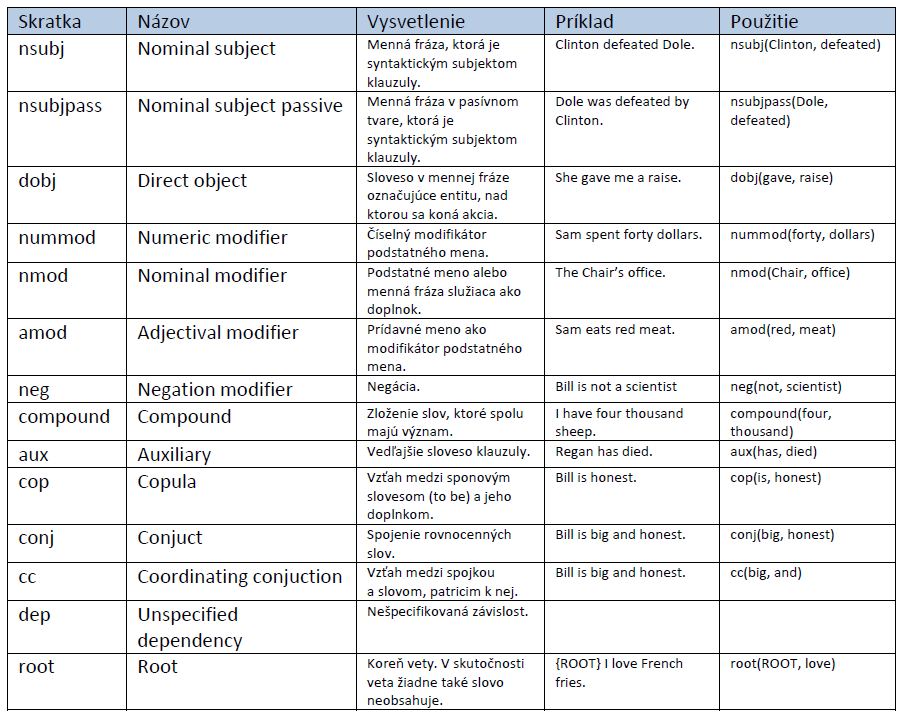
\includegraphics[scale=0.6]{dependencies_table}\end{center}
	\caption[Zoznam závislotí]{Zoznam závislostí}\label{fig:dependencies_table}
\end{figure}

\newpage
\ifthenelse {\boolean{bachelor}}
{
	%\section{Electronic medium}
	\section{Legenda diagramov kolekcií}
}
{
	%\chapter{Electronic medium}
	\chapter{Legenda diagramov kolekcií}
}
V priloženej tabuľke je legenda pre diagramy zobrazujúce štruktúru dát ukladaných v kolekciách v databáze.

\begin{figure}[H]
	\begin{center}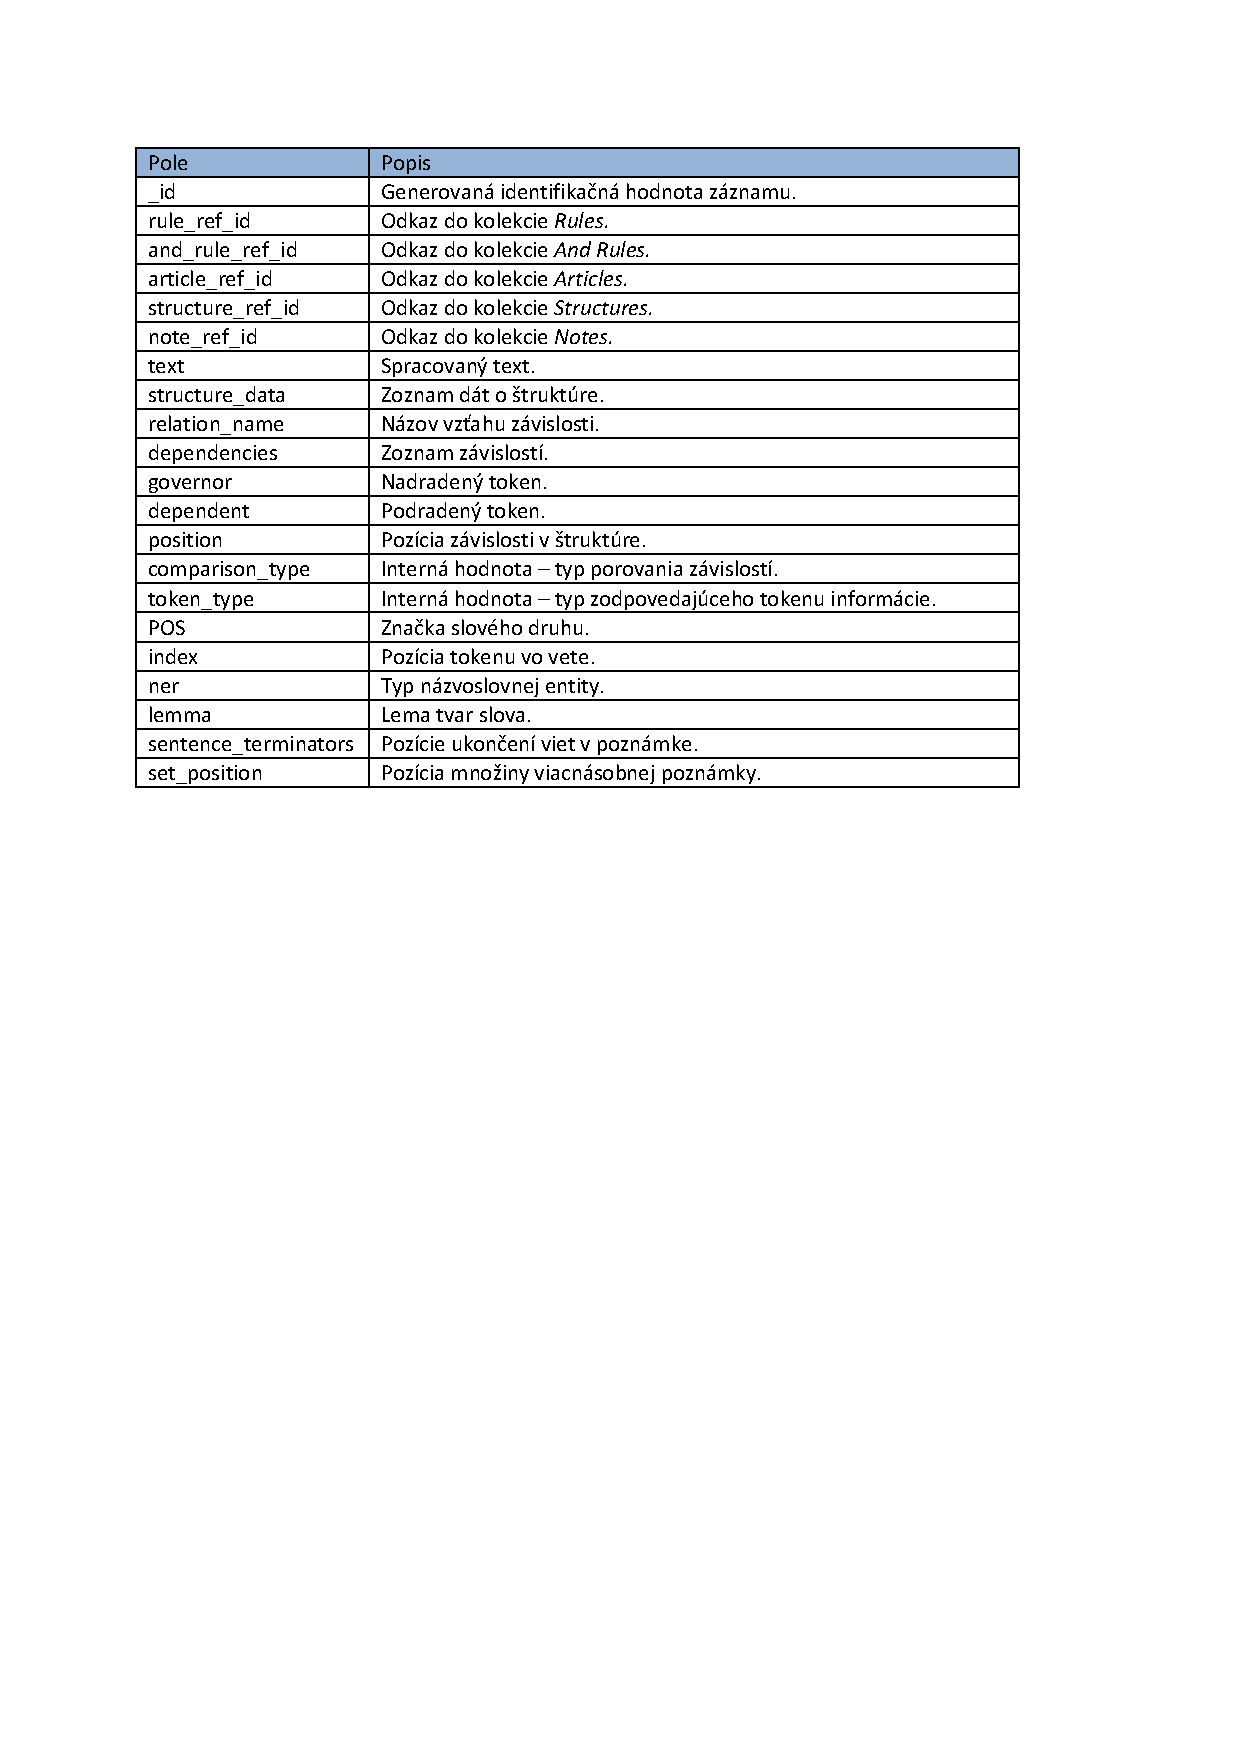
\includegraphics[scale=0.40]{collections_legend}\end{center}
	\caption[Legenda diagramov kolekcií]{Legenda diagramov kolekcií}\label{fig:collections_legend}
\end{figure}

\newpage
\ifthenelse {\boolean{bachelor}}
{
	%\section{Electronic medium}
	\section{Ukážka celého záznamu}
}
{
	%\chapter{Electronic medium}
	\chapter{Ukážka celého záznamu}
}
\label{appendix:db_entry_full_example}
V nasledujúcej ukážke je zobrazený celý záznam z databázy pre vetu ,,The president of the Czech Republic is Miloš Zeman.''. \\

\begin{lstlisting}[language = json, caption={Ukážka dát kolekcie rules}, label = {code:collection_rules_data_example}]
{
	"_id" : ObjectId("562d5aa22a085409d0bdba1d"),
	"originalSentence" : "The president of the Czech Republic is Milos Zeman.",
	"note" : "President is Zeman.",
	"createdBy" : 0,
	"articleId" : -1,
	"sentencesEnds" : [3],
	"originalDependencies" : [{
		"dependencyName" : "det",
		"dependencies" : [{
			"governor" : {
				"pos" : "NN",
				"index" : 2
			},
			"dependent" : {
				"pos" : "DT",
				"index" : 1
			},
			"position" : 0
		}, {
			"governor" : {
				"pos" : "NNP",
				"index" : 6
			},
			"dependent" : {
				"pos" : "DT",
				"index" : 4
			},
			"position" : 3
		}]
	}, {
		"dependencyName" : "nsubj",
		"dependencies" : [{
			"governor" : {
				"pos" : "NNP",
				"index" : 9
			},
			"dependent" : {
				"pos" : "NN",
				"index" : 2
			},
			"position" : 1
		}]
	}, {
		"dependencyName" : "case",
		"dependencies" : [{
			"governor" : {
				"pos" : "NNP",
				"index" : 6
			},
			"dependent" : {
				"pos" : "IN",
				"index" : 3
			},
			"position" : 2
		}]
	}, {
		"dependencyName" : "compound",
		"dependencies" : [{
			"governor" : {
				"pos" : "NNP",
				"index" : 6
			},
			"dependent" : {
				"pos" : "NNP",
				"index" : 5
			},
			"position" : 4
		}, {
			"governor" : {
				"pos" : "NNP",
				"index" : 9
			},
			"dependent" : {
				"pos" : "NNP",
				"index" : 8
			},
			"position" : 7
		}]
	}, {
		"dependencyName" : "nmod",
		"dependencies" : [{
			"governor" : {
				"pos" : "NN",
				"index" : 2
			},
			"dependent" : {
				"pos" : "NNP",
				"index" : 6
			},
			"position" : 5
		}]
	}, {
		"dependencyName" : "cop",
		"dependencies" : [{
			"governor" : {
				"pos" : "NNP",
				"index" : 9
			},
			"dependent" : {
				"pos" : "VBZ",
				"index" : 7
			},
			"position" : 6
		}]
	}, {
		"dependencyName" : "root",
		"dependencies" : [{
			"governor" : {
				"pos" : "",
				"index" : -1
			},
			"dependent" : {
				"pos" : "NNP",
				"index" : 9
			},
			"position" : 8
		}]
	}],
	"noteDependencies" : [{
		"dependencyName" : "nsubj",
		"dependencies" : [{
			"governor" : {
				"pos" : "NNP",
				"index" : 9
			},
			"dependent" : {
				"pos" : "NN",
				"index" : 2
			},
			"position" : 0,
			"comparisonType" : 0
		}, {
			"governor" : {
				"pos" : "NNP",
				"index" : 9
			},
			"dependent" : {
				"pos" : "NN",
				"index" : 2
			},
			"position" : 2,
			"comparisonType" : 0
		}]
	}, {
		"dependencyName" : "cop",
		"dependencies" : [{
			"governor" : {
				"pos" : "NNP",
				"index" : 9
			},
			"dependent" : {
				"pos" : "VBZ",
				"index" : 7
			},
			"position" : 1
		}]
	}]
}
\end{lstlisting}
